\documentclass[12pt]{article}
\usepackage{graphicx}
\usepackage{epstopdf}
%
% Title[Enter title of the experiment here]
\title{EE230:experiment No.6\\
Non-idealities of opamp measurement}

% Author[Enter details of author here]
\author{Mudavtah vishnuvardhan,200070044}

% begin the document.
\begin{document}

% make a title page.[this creates title page]
\maketitle


\section{Overview of the experiment} %[This segment creates Section as seen in document]

\subsection{Aim of the experiment}%[This segment creates sebsections under the same section]
1.To measure offset voltage of a non ideal opamp\\
2.To measure bias currents and offset current of non-ideal opamp\\
3.Meaurement of DC open loop gain \(A_{ol}\)\\
\newpage
\subsection{Method}
\subsubsection{measurement of offset voltage (\(V_{os}\))}
\begin{figure}[h!]
\centering
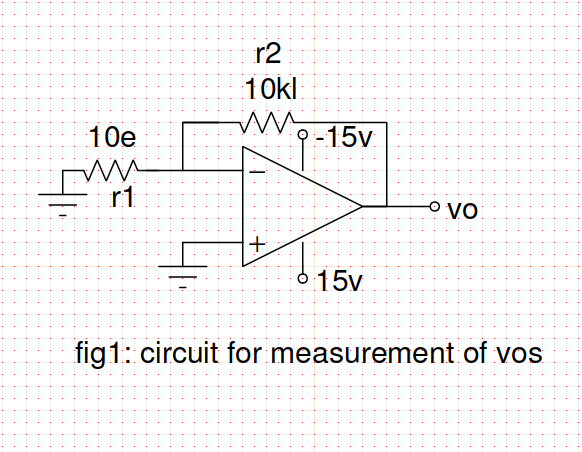
\includegraphics[scale = 0.5]{q1a_1.png}
\end{figure}
circuit is connected as shown in figure , now for measurement of \(v_{os}\) we use this formula :\\
\(v_{os}=V_{0}/(1+R_{2}/R_{1})\)\\
For measurement we have done we got values for \(V_{0}\) as 1.09v,thus\\
\(v_{os}=1.08v/(1+10k/10)=1.09mv\)\\
In the datasheet ,typical value=1mv and max possible value=5mv and hence we can say that our possible value is correct.
\newpage
\begin{figure}[h!]
\centering
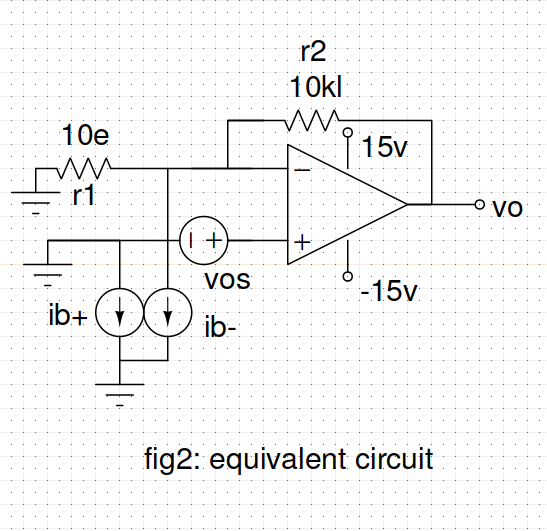
\includegraphics[scale = 0.6]{q1a_2.png}
\end{figure}
\newpage

\subsubsection{ measurement of inverting bias current (\(I_{B-}\))}
\begin{figure}[h!]
\centering
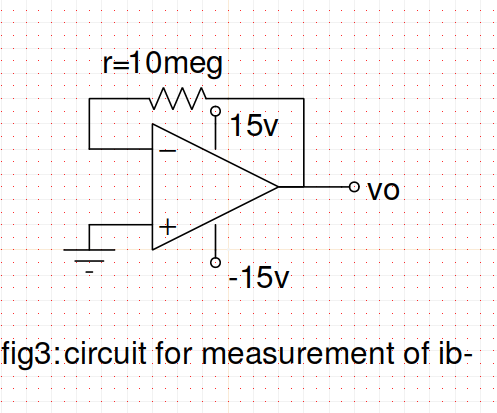
\includegraphics[scale = 0.5]{q1_b_cir.png}
\end{figure}
circuit is connected as shown in figure , now for measurement of \(I_{B-}\) we use this formula :\\
\(I_{B-}=V_{0}/R\)\\
For measurement we have done we got values for \(V_{0}\) as 3.37v,thus\\
\(I_{B-}=3.37/10^{7}=337nA\)\\
\newpage
\begin{figure}[h!]
\centering
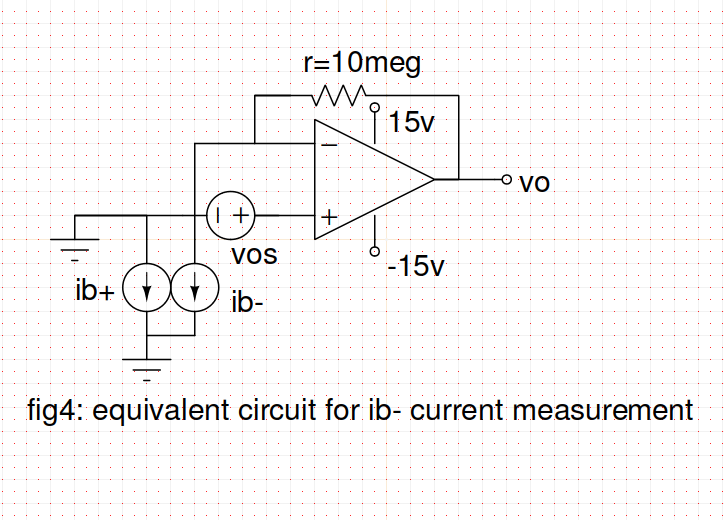
\includegraphics[scale = 0.6]{q1_b_ib-.png}
\end{figure}
\newpage

\subsubsection{ measurement of Non-inverting bias current (\(I_{B+}\))}
\begin{figure}[h!]
\centering
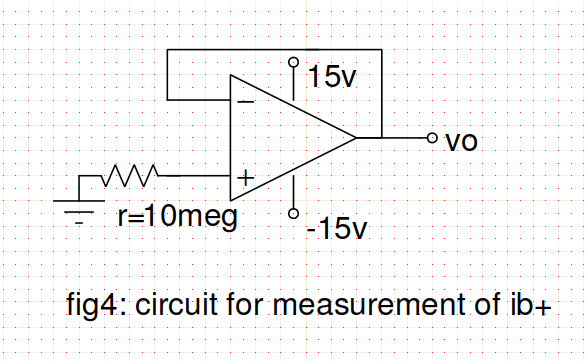
\includegraphics[scale = 0.5]{q1_c_cir.png}
\end{figure}
circuit is connected as shown in figure , now for measurement of \(I_{B+}\) we use this formula :\\
\(I_{B+}=V_{0}/R\)\\
For measurement we have done we got values for \(V_{0}\) as 3.92v,thus\\
\(I_{B-}=3.92/10^{7}=392nA\)\\
\newpage
\begin{figure}[h!]
\centering
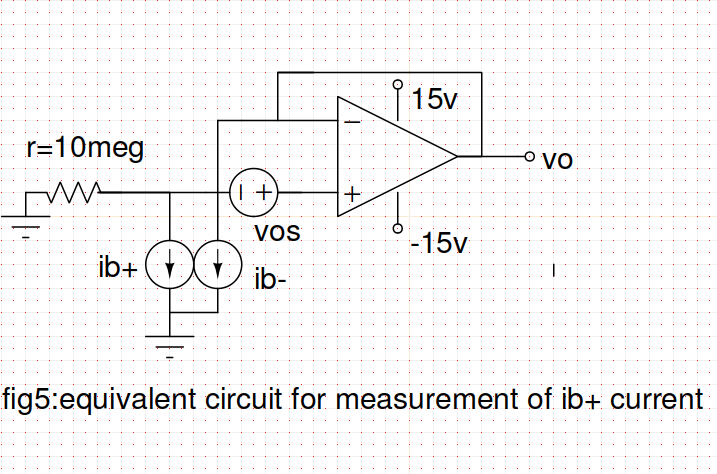
\includegraphics[scale = 0.6]{q1c_ib+.png}
\end{figure}
Typically these values are maximum 800nA as per the dataheet hence,we can conclude that our values match with datasheet.
\newpage
\subsubsection{ measurement of Open loop gain (\(A_{ol}\))}
\begin{figure}[h!]
\centering
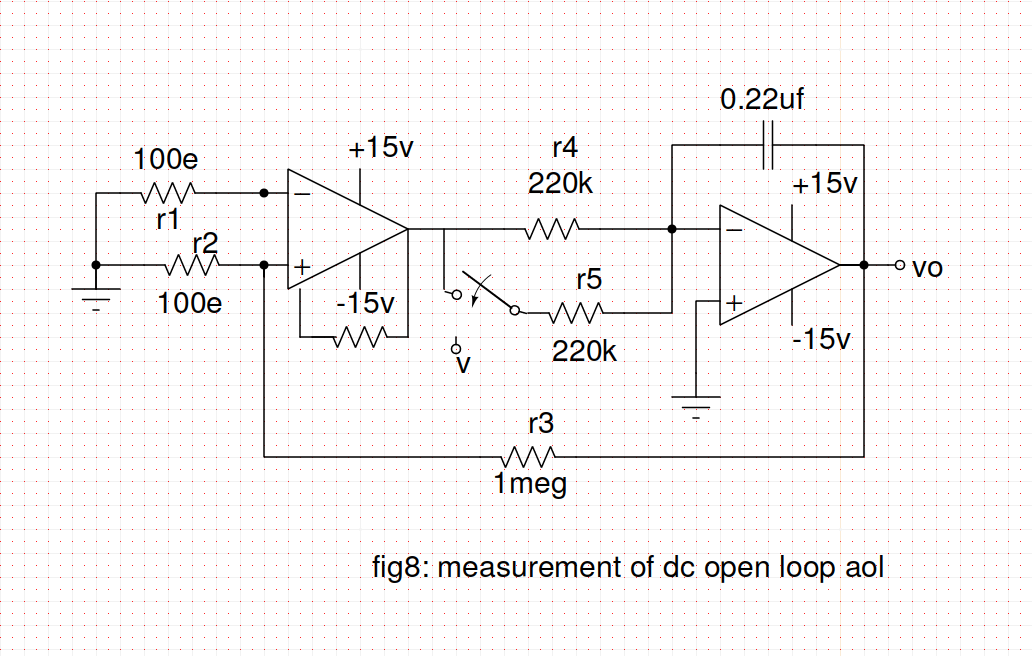
\includegraphics[scale = 0.4]{q2.png}
\end{figure}
circuit is connected as shown in figure , now for measurement of \(A_{ol}\) we use this formula :\\
\(A_{ol}=-V'*(R_{2}+R_{3}/R_{2}*(V_{oB}-V{oA}))\)\\
\(V_{oB}\) and \(V_{oA}\) are values obtained when the circuit is in position 1 and 2 respectively.\\
\textbf{Values obtained for \(V'=1v\):\\}
\(V_{oA}=0.05v\),\(V_{oB}=0.01v\) which gives us \(A_{ol}=2.5*10^{5}\).\\
\textbf{Values obtained for \(V'=2v\):\\}
\(V_{oA}=0.05v\),\(V_{oB}=-0.04v\) which gives us \(A_{ol}=2.22*10^{5}\).\\
\textbf{Values obtained for \(V'=3v\):\\}
\(V_{oA}=0.05v\),\(V_{oB}=-0.1v\) which gives us \(A_{ol}=2*10^{5}\).\\
Theoretically,\(A_{ol}=2*10^{5}\),hence we can say our values almost match the actual values.
\section{Experiment completion status}
I have completed all sections in Lab only.
\end{document}
